%%%%%%%%%%%%%%%%%%%%%%%%%%%%%%%%%%%%%%%%%%%%%%%%%%%%%%%%%%%%%%%%%%%%%%
% Lớp 11 | Hàm số lượng giác và phương trình lượng giác | Hàm số lượng giác và đồ thị
% Dạng 1D1?4-7: Bảng biến thiên và đồ thị
% Số câu: 14  (sinh tự động bởi tach_cau.py; từ nay thầy sửa trực tiếp file này)
%%%%%%%%%%%%%%%%%%%%%%%%%%%%%%%%%%%%%%%%%%%%%%%%%%%%%%%%%%%%%%%%%%%%%%

%%%%%%%%%%%%%%%% TRẮC NGHIỆM 4 PHƯƠNG ÁN %%%%%%%%%%%%%%%%

% nguồn: Ok_TracNghiemLop11_Lan1
\begin{ex}%[1D1N4-7]%[ma:db7b8347]
	Đồ thị của  hàm số nào có hình biểu diễn bên dưới đây?\\
	\pgfkeys{/pgfplots/Axis Style/.style={ 
	width=17.5cm, height=5cm, 
	axis  x line=center,
	axis  y line=middle,
	 samples=100,xlabel=$x$,
	ylabel=$y$, 
	ymin=-1.5,  ymax=1.5,
	xmin=-10.0, xmax=10.2, 
	 domain=-3*pi:3*pi
	 }}
	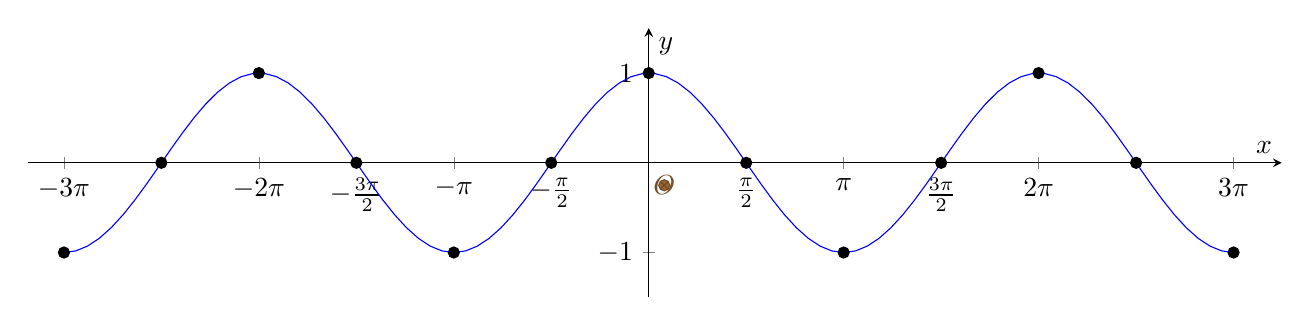
\begin{tikzpicture}
			\begin{axis}[
					declare  function={Y (\x)=cos (deg (\x));},
					Axis  Style,
					 xtick={
					 -9.424777,-6.28318,-4.7123889,-3.14159,-1.5708,
					 1.5708,3.14159,4.7123889,6.28318,9.424777
					 },
					xticklabels={ 
					$-3\pi$,$-2\pi$,$-\frac{3\pi}{2}$,$-\pi$,$-\frac{\pi}{2}$, 
					 $\frac{\pi}{2}$,$\pi$,$\frac{3\pi}{2}$,$2\pi$,$3\pi$
				} 
					 ]
				\addplot [mark=none,blue]  {Y (x)};
				\addplot [mark=*,only  marks,samples at={-9.424777,-7.85398,-6.28318,-4.7123889,-3.14159,-1.5708,0,1.5708,3.14159,4.7123889,6.28318,7.85398,9.424777}] {Y (x)};
				 \addplot coordinates {(0.25,-0.25)} node{$O$}{};
				\pgfplotsinvokeforeach{-4.7123889,-1.5708,1.5708,4.7123889}{\draw [dashed](axis cs:#1,{Y (#1)}) -- (axis cs:0,{Y (#1)})--(axis cs:#1,{Y (#1)}) --  (axis cs:#1,0);}
			\end{axis}
		\end{tikzpicture}
	 \choice
		{$y=\sin x$} 
		 {\True $y=\sin \left(\dfrac{\pi}{2}-x\right)$}
		 {$y=\sin 2x$}
		{$y=\cos 2x$} 
	 \loigiai{
		Ta có $y=\sin\left(\dfrac{\pi}{2}-x\right)=\cos x$. Đồ thị trên là của hàm  số $y=\cos x$.
	} 
\end{ex}

% nguồn: Ok_TracNghiemLop11_Lan1
\begin{ex}%[1D1N4-7]%[ma:f428931d]
	Cho  đồ thị hàm số $y=\sin x$ như hình vẽ sau
	\begin{center}
		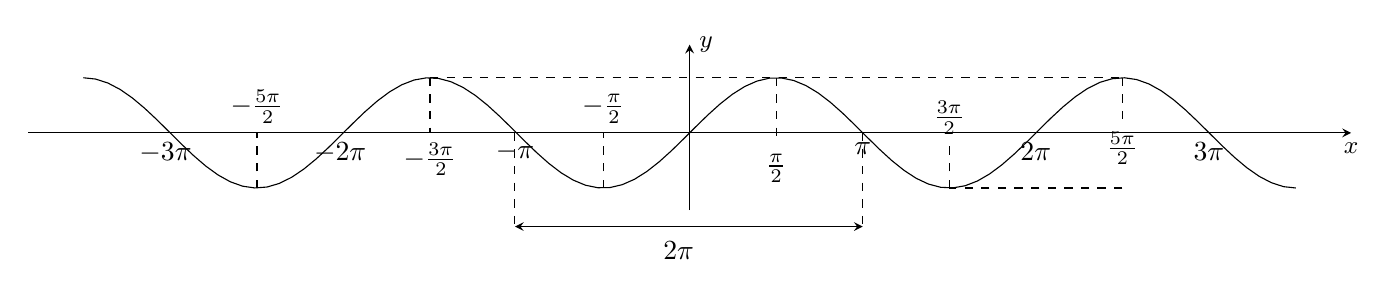
\begin{tikzpicture}[>=stealth,x=1cm,y=1cm,scale=0.7]
				 \draw[->] (-12,0) -- (12,0) node[below] {\small $x$};
				\draw[->] (0,-1.4) -- (0,1.6) node[right]  {\small $y$};
				\draw[samples=100,domain=-11:11] plot  (\x,{sin ((\x)*180/pi)});
				 \draw (-3.17,0) node[below] {$-\pi$};
				\draw (3.14,0) node[below]  {$\pi$};
				 \draw (-6.34,0) node[below] {$-2\pi$};
				 \draw (6.28,0) node[below] {$2\pi$};
				\draw (-9.51,0)  node[below] {$-3\pi$};
				\draw (9.42,0) node[below] {$3\pi$}; 
				\draw  (-0.2,-1.8) node[below] {$2\pi$};
				\draw[dashed] (-1.57,-1)--(-1.57,0) node[above]  {$-\frac{\pi}{2}$};
				 \draw[dashed] (1.57,1)--(1.57,-0.2) node[below] {$\frac{\pi}{2}$};
				\draw[dashed]  (-4.71,1)--(-4.71,0) node[below] {$-\frac{3\pi}{2}$};
				\draw[dashed] (4.71,-1)--(4.71,-0.2)  node[above] {$\frac{3\pi}{2}$};
				\draw[dashed]  (-7.85,-1)--(-7.85,0) node[above] {$-\frac{5\pi}{2}$};
				\draw[dashed] (7.85,1)--(7.85,0.2)  node[below] {$\frac{5\pi}{2}$};
				\draw[dashed] (-4.71,1)--(7.85,1); 
				 \draw[dashed] (--7.85,-1)--(4.71,-1)
					 (-3.17,0)--(-3.17,-1.8)
					 (3.14,0)--(3.14,-1.8);
				\draw[<->]  (-3.17,-1.7)--(3.14,-1.7);
			\end{tikzpicture}
	\end{center}
	Mệnh đề  nào đúng?
	 \choice
		{Hàm số $y=\sin x$ nghịch biến  trên $\left(\dfrac{-\pi}{2};\dfrac{\pi}{2}\right)$}
		{Hàm số $y=\sin x$ đồng biến trên  $\left(\dfrac{\pi}{2};\dfrac{3\pi}{2}\right)$}
		{Hàm số $y=\sin x$ đồng biến trên  $\left(\dfrac{-3\pi}{2};-\pi\right)$}
		{\True Hàm số $y=\sin x$ đồng biến trên  $\left(-\dfrac{\pi}{2}; 0\right)$}
	\loigiai{ 
	Hàm số $y=\sin x$ đồng biến $\left(-\dfrac{\pi}{2};0\right)$.} 
\end{ex}

% nguồn: Ok_TracNghiemLop11_Lan1
\begin{ex}%[1D1N4-7]%[ma:97881519]
	Cho hàm số $y=f(x)$ có đồ thị như hình  vẽ sau.
	\begin{center}
		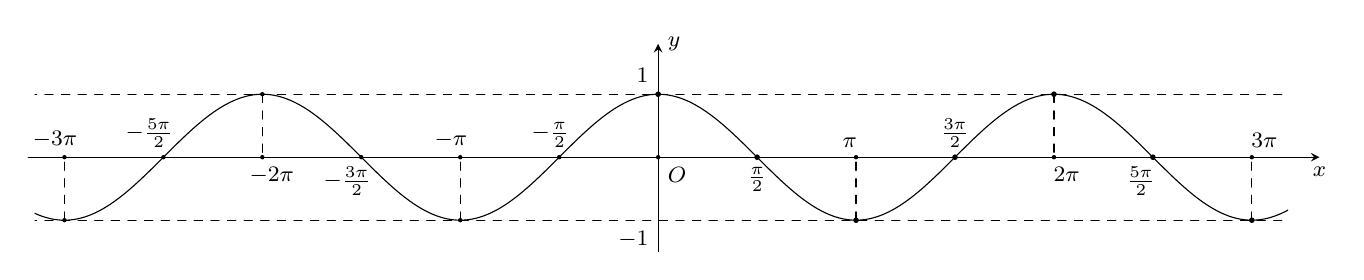
\begin{tikzpicture}[scale=0.8,>=stealth,font=\footnotesize,line join=round,line cap=round]
				\def\xmin{-10} \def\xmax{10.5} \def\ymin{-1.5} \def\ymax{1.8} 
				\draw[->] (\xmin,0)--(\xmax,0) node  [below]{$x$};
				 \draw[->] (0,\ymin)--(0,\ymax) node [right]{$y$};
				\fill (0,0) circle (1pt) node  [below right]{$O$};
				 \clip (\xmin+0.1,\ymin) rectangle (\xmax-0.5,\ymax-0.15);
				\draw[smooth,samples=400,domain=\xmin:\xmax] plot (\x,{cos  (\x r)});
				 \draw[dashed] (\xmin,1)--(\xmax,1)
					 (\xmin,-1)--(\xmax,-1);
				\foreach  \x in {-3*pi,-2.5*pi,-2*pi,-1.5*pi,-pi,-0.5*pi,0}
					{\fill (\x,cos \x*180/pi) circle (1pt); 
				\draw[dashed]  (\x,cos \x*180/pi)--(\x,0);
				\draw[fill]  (-\x,cos -\x*180/pi) circle (1pt);
				\draw[dashed] (-\x,cos \x*180/pi)--(-\x,0);} 
				\foreach \x  in {-3*pi,-2*pi,-pi,pi,2*pi,3*pi}
				\fill (\x,0) circle (1pt); 
				\node at (0,1.3)  [left]{$1$};
				\node at (0,-1.3)  [left]{$-1$};
				\node at  (-2*pi+0.15,0) [below]{$-2\pi$};
				 \node at (-3*pi-0.15,0) [above]{$-3\pi$};
				 \node at (-2.4*pi,0) [above left]{$-\frac{5\pi}{2}$};
				\node  at (-1.4*pi,0) [below left]{$-\frac{3\pi}{2}$};
				 \node at (-pi-0.15,0) [above]{$-\pi$};
				\node at (-0.4*pi,0)  [above left]{$-\frac{\pi}{2}$};
				\node at (0.5*pi,0)  [below]{$\frac{\pi}{2}$};
				\node at (pi-0.1,0) [above]{$\pi$}; 
				\node  at (1.5*pi,0) [above]{$\frac{3\pi}{2}$};
				\node at (2*pi+0.2,0) [below]{$2\pi$}; 
				 \node at (2.5*pi+0.2,0) [below left]{$\frac{5\pi}{2}$};
				\node  at (3*pi+0.2,0) [above]{$3\pi$};
			\end{tikzpicture}
	\end{center}
	Khẳng định nào sau đây  đúng về hàm số $y=f(x)$?
	\choice 
		{Đồ thị trên là đồ thị của hàm  số $y=\sin x$}
		{\True Hàm  số $y=f(x)$ nghịch biến trên khoảng $\left(\dfrac{\pi}{2};\pi\right)$}
		{Đồ thị trên là đồ  thị của hàm số $y=\tan x$}
		{Hàm  số $y=f(x)$ đồng biến trên khoảng $\left(0;\dfrac{\pi}{2}\right)$}
	\loigiai{ Dựa vào đồ thị  ta thấy hàm số $y=f(x)$ nghịch biến trên khoảng $\left(\dfrac{\pi}{2};\pi\right)$.
	 }
\end{ex}

% nguồn: Ok_TracNghiemLop11_Lan1
\begin{ex}%[1D1N4-7]%[ma:23c952e3]
	Đồ thị của hàm số $y=\sin  \left( x+\dfrac{\pi }{4} \right)$ đi qua điểm nào sau đây?
	\choice 
		{$M\left( \dfrac{\pi  }{4}\,;\,0 \right)$ }
		{\True $N\left( 0\,;\,\dfrac{\sqrt{2}}{2} \right)$ } 
		{ $P\left(  \dfrac{\pi }{2}\,;\,1 \right)$}
		{$Q\left( 0\,;\,1  \right)$}
	 \loigiai{
	 Với $x=0\Rightarrow y=\sin \dfrac{\pi }{4}=\dfrac{\sqrt{2}}{2}$.}
\end{ex}

% nguồn: Ok_TracNghiemLop11_Lan1
\begin{ex}%[1D1H4-7]%[ma:a339c558]
	Dùng đồ thị hàm số $y=-\sin x$ (tham khảo hình vẽ), xác định số nghiệm của phương trình $2\sin x+\sqrt{2}=0$ trên đoạn  $-\dfrac{3\pi}{2} \le x\le \dfrac{3\pi}{2}$.
	\begin{center}
		\begin{tikzpicture}[line join=round,line cap=round,>=stealth,scale=1.25,transform shape]
				\pgfmathsetmacro{\xmin}{-1.5*pi} 
				 \pgfmathsetmacro{\xmax}{1.5*pi}
				\def\ymin{-1.5} \def\ymax{1.5}  \def\rt{.03}
				\draw[->](\xmin-.1,0)--(\xmax+1,0)  node[below]{$x$};
				\draw[->](0,-1.5)--(0,1.8)  node[left]{$y$};
				 \draw (0,0) node[below left]{$O$};
				\begin{scope}
					 \clip (\xmin,\ymin) rectangle (\xmax,\ymax);
					\draw[domain=\xmin:\xmax,samples=200,smooth] plot (\x,{-sin  (\x r)});
				\end{scope}
				\draw[dash  pattern=on 2pt off 1.5pt]
					(-pi,0) node[below]{$-\pi$} 
					(pi,0) node[below]{$\pi$} 
					(-1.5*pi,0)  node[above]{-$\tfrac{3\pi}{2}$}|-(0,-1) node[below left]{$-1$}
					(1.5*pi,0) node[below]{$\tfrac{3\pi}{2}$}|-(0,1)  node[above left]{$1$}
					 (-.5*pi,0) node[below]{-$\tfrac{\pi}{2}$}|-(0,1)
					(.5*pi,0) node[below  right]{$\tfrac{\pi}{2}$}|-(0,-1);
			\end{tikzpicture}
	\end{center}
	 \choice
		 {$2$}
		{\True  $3$}
		{$1$} 
		{$4$} 
	\loigiai{ 
		Ta có: $2\sin x-\sqrt{2}=0\Leftrightarrow-\sin x=\dfrac{\sqrt{2}}{2}$. Đồ thị hàm số $y=-\sin x$ và đường thẳng $y=\dfrac{\sqrt{2}}{2}$ trên đoạn $-\dfrac{3\pi}{2} \le x\le  \dfrac{3\pi}{2}$ được vẽ như hình sau:
		\begin{center}
			\begin{tikzpicture}[line join=round,line cap=round,>=stealth,scale=1.25,transform shape]
					\pgfmathsetmacro{\xmin}{-1.5*pi} 
					\pgfmathsetmacro{\xmax}{1.5*pi} 
					 \def\ymin{-1.5} \def\ymax{1.5} \def\rt{.03}
					\draw[->](\xmin-.1,0)--(\xmax+1,0)  node[below]{$x$};
					 \draw[->](0,-1.5)--(0,1.8) node[left]{$y$};
					\draw (0,0)  node[below left]{$O$};
					\begin{scope}
						 \clip (\xmin,\ymin) rectangle (\xmax,\ymax);
						\draw[domain=\xmin:\xmax,samples=200,smooth]  plot (\x,{-sin (\x r)});
					\end{scope}
					\draw[dash pattern=on 2pt off  1.5pt]
						(-pi,0)  node[below]{$-\pi$}
						 (pi,0) node[below]{$\pi$}
						(-1.5*pi,0) node[above]{-$\tfrac{3\pi}{2}$}|-(0,-1)  node[below left]{$-1$}
						(1.5*pi,0) node[below]{$\tfrac{3\pi}{2}$}|-(0,1) node[above  left]{$1$}
						 (-.5*pi,0) node[below]{-$\tfrac{\pi}{2}$}|-(0,1)
						(.5*pi,0)  node[below right]{$\tfrac{\pi}{2}$}|-(0,-1);
					 \draw[blue](\xmin+.75,.71)--(\xmax,.71) node[above,pos=.1]{$y=\tfrac{\sqrt{2}}{2}$};
				\end{tikzpicture}
		\end{center}
		Từ đồ  thị ta thấy đường thẳng $y=\dfrac{\sqrt{2}}{2}$ cắt đồ thị hàm số $y=-\sin x$ trên đoạn $-\dfrac{3\pi}{2} \le x\le \dfrac{3\pi}{2}$ tại 3 điểm.
	} 
\end{ex}

% nguồn: Ok_TracNghiemLop11_Lan1
\begin{ex}%[1D1H4-7]%[ma:24eddb5f]
	Hình vẽ bên  dưới là đồ thị của hàm số nào?
	\begin{center}
		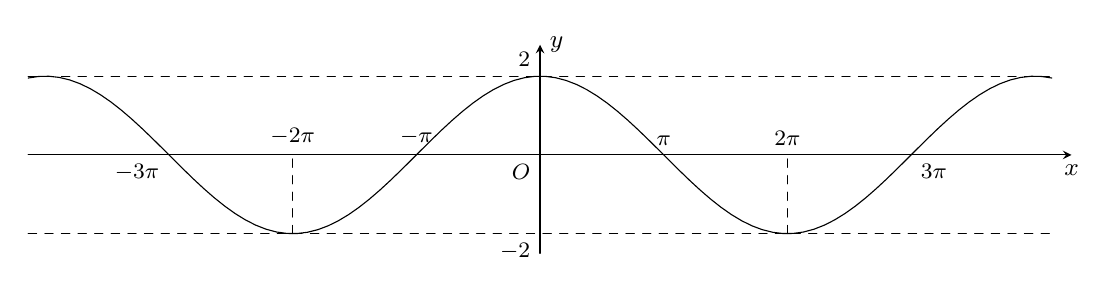
\begin{tikzpicture}[>=stealth,line join=round,line cap=round,font=\footnotesize,scale=0.5]
				\draw[->] (-13,0) --  (13.5,0) node[below] {\small $x$};
				\draw[->]  (0,-2.5) -- (0,2.8) node[right] {\small $y$};
				\draw[samples=100,domain=-13:13]  plot (\x,{2*cos ((\x)*90/pi)});
				\draw  (0,0) node [below left] {$O$};
				\draw  (0,2) node [above left] {$2$};
				\draw (0,-2) node [below left] {$-2$}; 
				 \draw (-pi,0) node[above] {$-\pi$};
				\draw (pi,0)  node[above] {$\pi$};
				\draw[dashed] (-2*pi,-2)--(-2*pi,0) node[above] {$-2\pi$}; 
				\draw[dashed]  (2*pi,-2)--(2*pi,0) node[above] {$2\pi$};
				\draw (-3*pi,0) node[below  left] {$-3\pi$};
				\draw (3*pi,0) node[below right] {$3\pi$}; 
				\draw[dashed] (-13,2)--(13,2); 
				 \draw[dashed] (-13,-2)--(13,-2);
			\end{tikzpicture}
	\end{center}
	\choice 
		{\True $y=2\cos  \dfrac{x}{2}$}
		{$y=\sin  x+2$}
		 {$y=2\sin \dfrac{x}{2}$}
		{$y=1+2\cos x$} 
	\loigiai{ 
		Thử điểm $\left( 0\,;\,1 \right)$ lần lượt vào các hàm số $y=2\cos \dfrac{x}{2}$, $y=\sin x+2$, $y=2\sin \dfrac{x}{2}$, $y=1+2\cos x$ thấy rằng điểm  $\left( 0\,;\,1 \right)$ không thuộc vào đồ thị hai hàm số $y=2\sin \dfrac{x}{2}$ và $y=1+2\cos x$.\\
		Thử điểm $\left( \pi \,;\,0 \right)$ vào hai hàm số $y=2\cos \dfrac{x}{2}$, $y=\sin x+2$ thấy rằng điểm $\left( \pi \,;\,0 \right)$ hông thuộc vào  đồ thị hàm số $y=1+2\cos x$.\\
	Vậy hình vẽ chỉ  có thể là đồ thị hàm số $y=2\cos \dfrac{x}{2}$.}
\end{ex}

% nguồn: Ok_TracNghiemLop11_Lan1
\begin{ex}%[1D1H4-7]%[ma:a09c1088]
	Cho đồ thị hàm số $f\left( x \right)$ như hình vẽ dưới đây. Hỏi tịnh tiến đồ thị hàm số $f\left( x \right)$ theo vectơ $\vec{v}=\left( \dfrac{\pi }{2};0 \right)$ thì được đồ thị hàm số 
	\begin{center}
		\begin{tikzpicture}[>=stealth,line join=round,line cap=round,font=\footnotesize,scale=0.8]
				\draw[->] (-6,0) -- (6.5,0) node[below] {\small  $x$};
				\draw[->] (0,-1.8) -- (0,2) node[right]  {\small $y$};
				\draw[samples=100,domain=-6:6] plot (\x,{cos ((\x)*180/pi)}); 
				\draw (0,0) node [below left] {$O$}; 
				\draw (0,1) node [above  left] {$1$};
				\draw (0,-1) node [below left]  {$-1$};
				\draw (-4.71,0) node[above] {$-\frac{3\pi}{2}$}; 
				\draw (4.71,0) node[above] {$\frac{3\pi}{2}$}; 
				\draw (-3.17,0) node[above]  {$-\pi$};
				 \draw (pi,0) node[above] {$\pi$};
				\draw[dashed] (-1.57,0)  node[below] {$-\frac{\pi}{2}$};
				\draw[dashed] (1.57,0)  node[below] {$\frac{\pi}{2}$};
				 \draw[dashed] (pi,0)--(pi,-1);
				\draw[dashed]  (-pi,0)--(-pi,-1);
			\end{tikzpicture}
	\end{center}
	 \choice
		{$y=\tan x$} 
		{\True $y=\sin x$} 
		 {$y=\cos x$}
		{$y=\cot x$} 
	\loigiai{ 
	Theo hình vẽ thì đồ thị trong hình là của hàm số $y=\cos x$. Khi tịnh tiến theo vectơ $\vec{v}=\left( \dfrac{\pi }{2};0  \right)$ thì ta được đồ thị của hàm số $y=\cos \left( x-\dfrac{\pi }{2} \right)=\sin x$.}
\end{ex}

% nguồn: Ok_TracNghiemLop11_Lan1
\begin{ex}%[1D1H4-7]%[ma:bb77d4f3]
	Cho hàm số $y=\cos x$ có đồ thị như hình vẽ. Tìm số nghiệm của phương trình $2\cos x+1=0$  trên khoảng $\left(0;\pi \right)$.
	\begin{center}
		\begin{tikzpicture}[line join=round,line cap=round,>=stealth,scale=1.25,transform shape]
				 \pgfmathsetmacro{\xmin}{0}
				\pgfmathsetmacro{\xmax}{pi} 
				 \def\ymin{-1.5} \def\ymax{1.5} \def\rt{.03}
				 \draw[->](\xmin-1,0)--(\xmax+1,0) node[below]{$x$};
				\draw[->](0,-1.5)--(0,1.8) node[left]{$y$}; 
				\draw (0,0) node[above  left]{$O$};
				\begin{scope}
					\clip (\xmin,\ymin) rectangle  (\xmax,\ymax);
					 \draw[domain=\xmin:\xmax,samples=200,smooth] plot (\x,{cos (\x r)});
				\end{scope}
				 \draw[dash pattern=on 2pt off 1.5pt]
					(0,1) node[above left]{$1$} 
					(pi,0) node[above]{$\pi$}|-(0,-1)  node[left]{$-1$};
			\end{tikzpicture}
	\end{center}
	\choice 
		 {$0$}
		{$2$} 
		{$3$} 
		 {\True $1$}
	 \loigiai{
		Ta có phương trình $2\cos  x+1=0\Leftrightarrow \cos x=-\dfrac{1}{2}$.\\
		Số nghiệm phương trình trên $\left(0;\pi \right)$  bằng số giao điểm của đồ thị hàm số $y=\cos x$ với đường thẳng $y=-\dfrac{1}{2}$ trên $\left(0;\pi \right)$.
		\begin{center}
			\begin{tikzpicture}[line join=round,line cap=round,>=stealth,scale=1.25,transform shape]
					 \pgfmathsetmacro{\xmin}{0}
					\pgfmathsetmacro{\xmax}{pi} 
					\def\ymin{-1.5}  \def\ymax{1.5} \def\rt{.03}
					\draw[->](\xmin-1,0)--(\xmax+1,0)  node[above]{$x$};
					\draw[->](0,-1.5)--(0,1.8)  node[left]{$y$};
					\draw  (0,0) node[above left]{$O$};
					\begin{scope}
						\clip (\xmin,\ymin) rectangle (\xmax,\ymax); 
						\draw[domain=\xmin:\xmax,samples=200,smooth]  plot (\x,{cos (\x r)});
					\end{scope}
					\draw[dash pattern=on  2pt off 1.5pt]
						(0,1) node[above left]{$1$} 
						(pi,0)  node[above]{$\pi$}|-(0,-1) node[left]{$-1$};
					\draw[blue] (\xmin-1,-.5)--(\xmax+1,-.5) node[right]{$y=-\tfrac{1}{2}$}; 
				\end{tikzpicture}
		\end{center}
		Dựa vào đồ thị hàm số ta thấy đường thẳng $y=-\dfrac{1}{2}$ cắt đồ thị hàm  số $y=\cos x$ trên $\left(0;\pi \right)$ tại đúng 1 điểm. Vì thế phương trình đã cho có đúng 1 nghiệm thuộc $\left(0;\pi \right)$.
	 }
\end{ex}

% nguồn: Ok_TracNghiemLop11_Lan1
\begin{ex}%[1D1H4-7]%[ma:2341fb27]
	Đường cong  trong hình dưới đây là đồ thị của một hàm số trong bốn hàm số được liệt kê ở bốn phương án $A,\ B,\ C,\ D$
	\begin{center}
		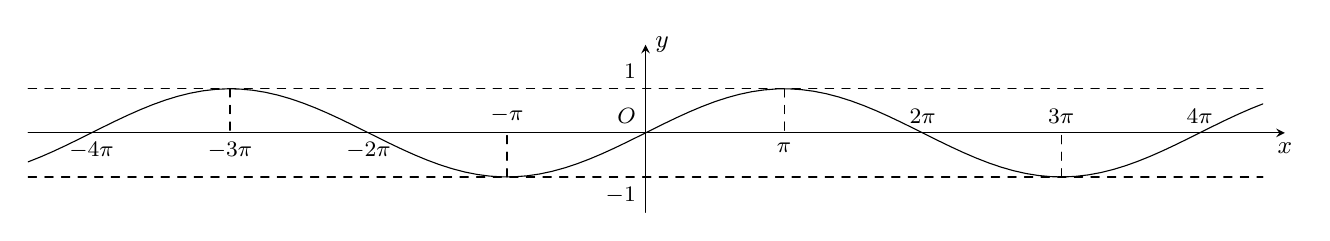
\begin{tikzpicture}[>=stealth,line join=round,line cap=round,font=\footnotesize,scale=0.56]
				\draw[->] (-14,0)  -- (14.5,0) node[below] {\small $x$};
				\draw[->] (0,-1.8) -- (0,2) node[right] {\small  $y$};
				\draw[samples=100,domain=-14:14]  plot (\x,{sin ((\x)*90/pi)});
				\draw (0,0) node [above left] {$O$}; 
				\draw (0,1) node  [above left] {$1$};
				\draw (0,-1) node  [below left] {$-1$};
				\draw (-2*pi,0)  node[below] {$-2\pi$};
				\draw (2*pi,0)  node[above] {$2\pi$};
				\draw (-4*pi,0) node[below]  {$-4\pi$};
				\draw (4*pi,0) node[above] {$4\pi$}; 
				 \draw[dashed] (-pi,-1)--(-pi,0) node[above] {$-\pi$};
				\draw[dashed] (pi,1)--(pi,0) node[below]  {$\pi$};
				\draw[dashed] (-3*pi,1)--(-3*pi,0) node[below]  {$-3\pi$};
				\draw[dashed] (3*pi,-1)--(3*pi,0) node[above] {$3\pi$}; 
				\draw[dashed]  (-14,1)--(14,1);
				 \draw[dashed] (-14,-1)--(14,-1);
			\end{tikzpicture}
	\end{center}
	Hỏi hàm số đó là hàm số nào? 
	\choice 
		{$y=\sin \dfrac{x}{2}$} 
		{$y=\cos  \dfrac{x}{2}$}
		{$y=-\cos \dfrac{x}{4}$} 
		{\True $y=\sin \left( -\dfrac{x}{2} \right)$} 
	\loigiai{ 
	Đồ thị hàm số đi qua điểm $\left( \pi;-1 \right)$ nên ta chọn hàm số $y=\sin \left( -\dfrac{x}{2} \right)$.} 
\end{ex}

% nguồn: Ok_TracNghiemLop11_Lan1
\begin{ex}%[1D1H4-7]%[ma:a7e09934]
	Dùng đồ thị hàm số $y=\sin x$ (tham  khảo hình vẽ) để xác định số nghiệm của phương trình $2\sin x-1=0$ trên khoảng $\left(-\dfrac{\pi}{2};2\pi \right)$.
	\begin{center}
		\begin{tikzpicture}[line join=round,line cap=round,>=stealth,scale=.95,transform shape]
				\pgfmathsetmacro{\xmin}{-.5*pi} 
				 \pgfmathsetmacro{\xmax}{2*pi}
				 \def\ymin{-1.5} \def\ymax{1.5} \def\rt{.03}
				\draw[->](\xmin-.1,0)--(\xmax+1,0)  node[below]{$x$};
				\draw[->](0,-1.5)--(0,1.8) node[left]{$y$}; 
				\draw (0,0) node[below  right]{$O$};
				\begin{scope}
					\clip (\xmin,\ymin) rectangle  (\xmax,\ymax);
					\draw[domain=\xmin:\xmax,samples=200,smooth] plot (\x,{sin (\x  r)});
				\end{scope}
				 \draw[dash pattern=on 2pt off 1.5pt]
					(2*pi,0) node[above left]{$2\pi$} 
					 (pi,0) node[below left]{$\pi$}
					 (1.5*pi,0) node[above]{$\tfrac{3\pi}{2}$}|-(0,-1) node[above left]{$-1$}
					 (-.5*pi,0) node[above]{-$\tfrac{\pi}{2}$}|-(0,-1)
					(.5*pi,0) node[below]{$\tfrac{\pi}{2}$}|-(0,1) node[left]{$1$}; 
			\end{tikzpicture}
	\end{center}
	\choice 
		 {$3$}
		{\True $2$} 
		 {$1$}
		{$4$} 
	\loigiai{ 
		Ta có $2\sin  x-1=0\Leftrightarrow \sin x=\dfrac{1}{2}$.
		\begin{center}
			\begin{tikzpicture}[line join=round,line cap=round,>=stealth,scale=.95,transform shape]
					\pgfmathsetmacro{\xmin}{-.5*pi} 
					\pgfmathsetmacro{\xmax}{2*pi} 
					\def\ymin{-1.5}  \def\ymax{1.5} \def\rt{.03}
					 \draw[->](\xmin-.1,0)--(\xmax+1,0) node[below]{$x$};
					\draw[->](0,-1.5)--(0,1.8) node[left]{$y$}; 
					\draw (0,0) node[below  right]{$O$};
					\begin{scope}
						\clip  (\xmin,\ymin) rectangle (\xmax,\ymax);
						 \draw[domain=\xmin:\xmax,samples=200,smooth] plot (\x,{sin (\x r)});
					\end{scope}
					\draw[dash pattern=on 2pt  off 1.5pt]
						(2*pi,0) node[below right]{$2\pi$} 
						(pi,0)  node[below left]{$\pi$}
						(1.5*pi,0) node[below right]{$\tfrac{3\pi}{2}$}|-(0,-1)  node[above left]{$-1$}
						(-.5*pi,0) node[below  right]{-$\tfrac{\pi}{2}$}|-(0,-1)
						 (.5*pi,0) node[below]{$\tfrac{\pi}{2}$}|-(0,1) node[left]{$1$};
					\draw[blue] (\xmin,.5)--(\xmax,.5)  node[above left]{$y=\tfrac{1}{2}$};
				\end{tikzpicture}
		\end{center}
		Dựa vào đồ thị ta thấy đường thẳng $y=\dfrac{1}{2}$ cắt đồ thị  hàm số $y=\sin x$ tại hai điểm phân biệt.\\
		Vậy phương trình đã cho có hai  nghiệm phân biệt.
	} 
\end{ex}


%%%%%%%%%%%%%%%% ĐÚNG/SAI %%%%%%%%%%%%%%%%

% nguồn: Ok_dungsai_lop11_Lan1
\begin{ex}%[1D1H4-7]%[ma:468c35b5]
 Cho hàm số $y=\tan x$. Xét tính đúng-sai  của các phát biểu sau:
  \choiceTF
  {$y=\tan x$ là hàm  số lẻ, đồ thị đối xứng qua trục tung}
  {\True Đồ thị hàm số $y=\tan x$ có dạng\\ 
  \begin{center}
  \begin{tikzpicture}[line join=round,line cap=round,>=stealth,scale=.95,transform shape]
     \pgfmathsetmacro{\xmin}{-1.5*pi}
    \pgfmathsetmacro{\xmax}{1.5*pi} 
    \def\ymin{-3} \def\ymax{3}  \def\rt{.03}
     \draw[->](\xmin-.1,0)--(\xmax+1,0) node[below]{$x$};
    \draw[->](0,\ymin)--(0,\ymax+.5) node[left]{$y$}; 
    \draw (0,0)  node[below right]{$O$};
    \foreach \i in {-1,0,1}{ 
     \pgfmathsetmacro{\batdau}{\i*pi-1.25} 
     \pgfmathsetmacro{\left}{(\i-0.5)*pi} 
     \pgfmathsetmacro{\ketthuc}{\i*pi+1.25} 
      \draw[dashed,thin] (\left,\ymin)--(\left,\ymax);
     \draw[domain=\batdau:\ketthuc,samples=100,smooth,semithick]  plot (\x,{tan (\x r)});
     }
    \draw[dashed,thin] (1.5*pi,\ymin)--(1.5  * pi,\ymax);
    \draw[dash  pattern=on 2pt off 1.5pt,thin]
      (-pi,0) node[above]{-$\pi$}
     (pi,0) node[above]{$\pi$}; 
   \end{tikzpicture}
  \end{center}
  } 
  {Đồ thị hàm số $y=\tan  x$ cắt trục hoành tại 3 điểm có hoành độ trong $\left(0;2\pi \right)$}
  {$x=2$  là hoành độ giao điểm của hai đồ thị $y=\tan x$ và $y=2\tan x+\sqrt{3}$}
 \loigiai{ 
  \begin{itemchoice}
   \itemch $y=\tan x$ là hàm  số lẻ, đồ thị đối xứng qua gốc toạ độ
   \itemch  $y=\tan x$ đồ thị có dạng sau:
   \begin{center}
    \begin{tikzpicture}[line join=round,line cap=round,>=stealth,scale=.95,transform shape]
       \pgfmathsetmacro{\xmin}{-1.5*pi}
      \pgfmathsetmacro{\xmax}{1.5*pi} 
      \def\ymin{-3} \def\ymax{3} \def\rt{.03} 
      \draw[->](\xmin-.1,0)--(\xmax+1,0) node[below]{$x$}; 
      \draw[->](0,\ymin)--(0,\ymax+.5) node[left]{$y$}; 
      \draw (0,0)  node[below right]{$O$};
       \foreach \i in {-1,0,1}{
      \pgfmathsetmacro{\batdau}{\i*pi-1.25} 
      \pgfmathsetmacro{\left}{(\i-0.5)*pi} 
       \pgfmathsetmacro{\ketthuc}{\i*pi+1.25}
      \draw[dashed,thin]  (\left,\ymin)--(\left,\ymax);
      \draw[domain=\batdau:\ketthuc,samples=100,smooth,semithick] plot (\x,{tan  (\x r)});
       }
      \draw[dashed,thin] (1.5*pi,\ymin)--(1.5 *  pi,\ymax);
      \draw[dash pattern=on  2pt off 1.5pt,thin]
       (-pi,0) node[above]{-$\pi$}
      (pi,0) node[above]{$\pi$}; 
     \end{tikzpicture}
   \end{center}
   \itemch Đồ thị hàm số $y=\tan x$  cắt trục hoành tại 3 điểm có hoành độ trong $\left(0;2\pi \right)$.\\
   Xét phương  trình hoành độ giao điểm $\tan x=0\Leftrightarrow x=k\pi \left(k\in \mathbb{Z}\right)$.\\
   Trong khoảng $\left(0;2\pi  \right)$ ta có một nghiệm là $x=\pi$.
   \itemch $x=2$ là hoành độ  giao điểm của hai đồ thị $y=\tan x$ và $y=2\tan x+\sqrt{3}$.\\
   Phương trình hoành  độ giao điểm đồ thị hàm số $y=\tan x$ và $y=2\tan x+\sqrt{3}$ là
   \allowdisplaybreaks 
   \begin{eqnarray*}
    &&\tan x=2\tan x+\sqrt{3} \\ 
    &\Leftrightarrow& \tan x=\sqrt{3} \\ 
    &\Leftrightarrow& \tan x=\tan  \dfrac{\pi}{3}\\
    &\Leftrightarrow& x=\dfrac{\pi}{3}+k\pi \left(k\in  \mathbb{Z}\right).
   \end{eqnarray*}
   Với $x=2$ ta có $2=\dfrac{\pi}{3}+k\pi \Leftrightarrow  k=\dfrac{6-\pi}{3\pi} \notin \mathbb{Z}$.
  \end{itemchoice}
  }
\end{ex}

% nguồn: Ok_dungsai_lop11_Lan1
\begin{ex}%[1D1H4-7]%[ma:5edc6cd2]
 Cho hàm số $y=\cot x$. Xét  tính đúng-sai của các phát biểu sau:
 \choiceTF 
  {$y=\cot x$ là hàm số lẻ, đồ thị đối  xứng qua trục tung}
  {\True Đồ thị hàm số $y=\cot x$ có  dạng:\\
  \begin{tikzpicture}[line join=round,line cap=round,>=stealth,scale=.85,transform shape]
     \pgfmathsetmacro{\xmin}{-pi}
     \pgfmathsetmacro{\xmax}{2*pi}
    \def\ymin{-3} \def\ymax{3} \def\rt{.03} 
     \draw[->](\xmin-.1,0)--(\xmax+1,0) node[below]{$x$};
    \draw[->](0,\ymin)--(0,\ymax+.5)  node[left]{$y$};
    \draw  (0,0) node[below right]{$O$};
    \foreach \i in {-1,0,1}{ 
     \pgfmathsetmacro{\batdau}{\i*pi+.32} 
     \pgfmathsetmacro{\left}{\i*pi} 
     \pgfmathsetmacro{\ketthuc}{(\i+1)*pi-.32} 
     \draw[dashed,thin]  (\left,\ymin)--(\left,\ymax);
     \draw[domain=\batdau:\ketthuc,samples=100,smooth,red] plot  (\x,{cot (\x r)});
     }
     \draw[dashed,thin] (2*pi,\ymin)--(2 * pi,\ymax);
    \draw[dash pattern=on 2pt off  1.5pt,thin]
     (-.5*pi,0)  node[below]{-$\tfrac{\pi}{2}$}
     (1.5*pi,0) node[below]{$\tfrac{3\pi}{2}$} 
     (.5*pi,0)  node[below]{$\tfrac{\pi}{2}$};
   \end{tikzpicture}
  } 
  {Đồ  thị hàm số $y=\cot x$ cắt trục hoành tại 3 điểm có hoành độ trong $\left(0;2\pi \right)$}
  {$x=2$ là hoành độ giao điểm của hai đồ  thị $y=\cot x$ và $y=2\cot x-\sqrt{3}$}
  \loigiai{
  \begin{itemchoice}
   \itemch $y=\cot x$ là hàm số lẻ, đồ thị đối  xứng qua gốc toạ độ
   \itemch $y=\cot x$ đồ thị  có dạng sau:
   \begin{center}
    \begin{tikzpicture}[line join=round,line cap=round,>=stealth,scale=.85,transform shape]
      \pgfmathsetmacro{\xmin}{-pi} 
       \pgfmathsetmacro{\xmax}{2*pi}
      \def\ymin{-3} \def\ymax{3} \def\rt{.03} 
      \draw[->](\xmin-.1,0)--(\xmax+1,0) node[below]{$x$}; 
      \draw[->](0,\ymin)--(0,\ymax+.5)  node[left]{$y$};
      \draw  (0,0) node[below right]{$O$};
      \foreach \i in  {-1,0,1}{
      \pgfmathsetmacro{\batdau}{\i*pi+.32} 
       \pgfmathsetmacro{\left}{\i*pi}
       \pgfmathsetmacro{\ketthuc}{(\i+1)*pi-.32}
      \draw[dashed,thin]  (\left,\ymin)--(\left,\ymax);
      \draw[domain=\batdau:\ketthuc,samples=100,smooth,red] plot (\x,{cot (\x  r)});
      } 
       \draw[dashed,thin] (2*pi,\ymin)--(2 * pi,\ymax);
      \draw[dash pattern=on 2pt off 1.5pt,thin] 
      (-.5*pi,0)  node[below]{-$\tfrac{\pi}{2}$}
       (1.5*pi,0) node[below]{$\tfrac{3\pi}{2}$}
      (.5*pi,0)  node[below]{$\tfrac{\pi}{2}$};
     \end{tikzpicture}
   \end{center}
   \itemch Đồ thị hàm số $y=\cot x$ cắt  trục hoành tại 3 điểm có hoành độ trong $\left(0;2\pi \right)$.\\
   Xét phương trình hoành độ giao điểm $\cot x=0\Leftrightarrow x=\dfrac{\pi}{2}+k\pi \left(k\in \mathbb{Z}\right)$.\\ 
   Trong khoảng $\left(0;2\pi \right)$ ta có hai nghiệm là  $x=\dfrac{\pi}{2}\vee x=\dfrac{3\pi}{2}$.
   \itemch $x=2$ là hoành độ giao điểm của hai đồ  thị $y=\cot x$ và $y=2\cot x+\sqrt{3}$.\\
   Phương trình hoành độ giao điểm đồ thị hàm số $y=\cot x$ và $y=2\cot x-\sqrt{3}$ là 
   \allowdisplaybreaks 
   \begin{eqnarray*}
    &&\cot x=2\cot  x-\sqrt{3} \\
    &\Leftrightarrow& \cot  x=\sqrt{3} \\
    &\Leftrightarrow&  \cot x=\cot \dfrac{\pi}{6} \\
    &\Leftrightarrow& x=\dfrac{\pi}{6}+k\pi \left(k\in \mathbb{Z}\right). 
   \end{eqnarray*}
   Với $x=2$ ta có: $2=\dfrac{\pi}{6}+k\pi  \Leftrightarrow k=\dfrac{12-\pi}{6\pi} \notin \mathbb{Z}$.
  \end{itemchoice}
 } 
\end{ex}


%%%%%%%%%%%%%%%% TRẢ LỜI NGẮN %%%%%%%%%%%%%%%%

% nguồn: Ok_TraLoiNgan_Lop11_Lan2
\begin{ex}%[1D1V4-7]%[ma:bc4d31a6]
 Một con lắc lò xo dao động điều hoà quanh vị trí  cân bằng theo phương trình
 \begin{center}
 $y=25\sin  4\pi t$
 \end{center}
 ở đó $y$ được tính bằng centimét còn thời gian $t$ được tính bằng giây. Gọi $a$ là chu kì dao động của con lắc lò xo; $b$ (Hz) là tần số dao động của con lắc, tức là số lần dao động trong một giây và $c$ (cm) là khoảng cách giữa điểm cao nhất và  thấp nhất của con lắc. Tính $a+b+c$.
	 \shortans{52,5}
	\loigiai{ 
		Hàm  số $y=25\sin 4\pi t$ tuần hoàn với chu kì $T=\dfrac{2\pi}{4\pi}=\dfrac{1}{2}$.\\
		Suy ra chu kì dao  động của con lắc lò xo (tức là khoảng thời gian để con lắc thực hiện được một dao động toàn phần) là $T=\dfrac{1}{2}$ giây nên $a=0{,}5$.\\
		Vì chu kì dao động của con lắc là  $T = \frac{1}{2}$ giây nên trong $1$ giây con lắc thực hiện được $2$ dao
		động.\\ 
		Tức là tần số dao động của con lắc là $b =  f = \dfrac{1}{T} = 2$ (Hz).\\
		Vì phương trình dao động của con lắc là $y = 25\sin4\pi t$  nên biên độ dao động của nó là $A = 25$ (cm).\\
		Từ đó khoảng cách giữa điểm cao nhất và điểm thấp nhất của con lắc là $c =  2A = 50$ (cm).\\
		Vậy $a+b+c =  0{,}5+2+50 = 52{,}5$.
	} 
\end{ex}

% nguồn: Ok_TraLoiNgan_Lop11_Lan2
\begin{ex}%[1D1V4-7]%[ma:b727cafa]
	Giả sử khi một cơn sóng biển đi qua một cái cọc ở ngoài khơi, chiều cao của nước được mô hình hoá bởi hàm số $h(t)=90\cos\left(\dfrac{\pi}{10}t\right)$, trong đó $h(t)$ là độ cao tính bằng centimét trên mực nước biển trung bình tại thời điểm $t$ giây. Tìm chiều cao (đơn vị: cm) của sóng, tức là khoảng cách theo phương thẳng đứng giữa  đáy và đỉnh của sóng.
	 \shortans{90}
	 \loigiai{
		 Chu kì của sóng là $T=\dfrac{2\pi}{\dfrac{\pi}{10}}=20$ (giây).\\
		Chiều cao của sóng tức là chiều cao  của nước đạt được trong một chu kì dao động.\\
		Ta có $h(20)=90\cos\left(\dfrac{\pi}{10}\cdot  20\right)=90\cos(2\pi)=90$ (cm).\\
		 Vậy chiều cao của sóng là $90$ cm.
	 }
\end{ex}
